% Options for packages loaded elsewhere
\PassOptionsToPackage{unicode}{hyperref}
\PassOptionsToPackage{hyphens}{url}
%
\documentclass[
  12pt,
]{article}
\usepackage{lmodern}
\usepackage{amsmath}
\usepackage{ifxetex,ifluatex}
\ifnum 0\ifxetex 1\fi\ifluatex 1\fi=0 % if pdftex
  \usepackage[T1]{fontenc}
  \usepackage[utf8]{inputenc}
  \usepackage{textcomp} % provide euro and other symbols
  \usepackage{amssymb}
\else % if luatex or xetex
  \usepackage{unicode-math}
  \defaultfontfeatures{Scale=MatchLowercase}
  \defaultfontfeatures[\rmfamily]{Ligatures=TeX,Scale=1}
\fi
% Use upquote if available, for straight quotes in verbatim environments
\IfFileExists{upquote.sty}{\usepackage{upquote}}{}
\IfFileExists{microtype.sty}{% use microtype if available
  \usepackage[]{microtype}
  \UseMicrotypeSet[protrusion]{basicmath} % disable protrusion for tt fonts
}{}
\makeatletter
\@ifundefined{KOMAClassName}{% if non-KOMA class
  \IfFileExists{parskip.sty}{%
    \usepackage{parskip}
  }{% else
    \setlength{\parindent}{0pt}
    \setlength{\parskip}{6pt plus 2pt minus 1pt}}
}{% if KOMA class
  \KOMAoptions{parskip=half}}
\makeatother
\usepackage{xcolor}
\IfFileExists{xurl.sty}{\usepackage{xurl}}{} % add URL line breaks if available
\IfFileExists{bookmark.sty}{\usepackage{bookmark}}{\usepackage{hyperref}}
\hypersetup{
  pdftitle={Policing for Profit and the Mobilization of Black Voters},
  pdfauthor={Jonathan Ben-Menachem; Kevin Morris},
  hidelinks,
  pdfcreator={LaTeX via pandoc}}
\urlstyle{same} % disable monospaced font for URLs
\usepackage[margin=1in]{geometry}
\usepackage{longtable,booktabs}
\usepackage{calc} % for calculating minipage widths
% Correct order of tables after \paragraph or \subparagraph
\usepackage{etoolbox}
\makeatletter
\patchcmd\longtable{\par}{\if@noskipsec\mbox{}\fi\par}{}{}
\makeatother
% Allow footnotes in longtable head/foot
\IfFileExists{footnotehyper.sty}{\usepackage{footnotehyper}}{\usepackage{footnote}}
\makesavenoteenv{longtable}
\usepackage{graphicx}
\makeatletter
\def\maxwidth{\ifdim\Gin@nat@width>\linewidth\linewidth\else\Gin@nat@width\fi}
\def\maxheight{\ifdim\Gin@nat@height>\textheight\textheight\else\Gin@nat@height\fi}
\makeatother
% Scale images if necessary, so that they will not overflow the page
% margins by default, and it is still possible to overwrite the defaults
% using explicit options in \includegraphics[width, height, ...]{}
\setkeys{Gin}{width=\maxwidth,height=\maxheight,keepaspectratio}
% Set default figure placement to htbp
\makeatletter
\def\fps@figure{htbp}
\makeatother
\setlength{\emergencystretch}{3em} % prevent overfull lines
\providecommand{\tightlist}{%
  \setlength{\itemsep}{0pt}\setlength{\parskip}{0pt}}
\setcounter{secnumdepth}{5}
\usepackage{rotating}
\usepackage{setspace}
\usepackage{booktabs}
\usepackage{longtable}
\usepackage{array}
\usepackage{multirow}
\usepackage{wrapfig}
\usepackage{float}
\usepackage{colortbl}
\usepackage{pdflscape}
\usepackage{tabu}
\usepackage{threeparttable}
\usepackage{threeparttablex}
\usepackage[normalem]{ulem}
\usepackage{makecell}
\usepackage{xcolor}
\ifluatex
  \usepackage{selnolig}  % disable illegal ligatures
\fi
\newlength{\cslhangindent}
\setlength{\cslhangindent}{1.5em}
\newlength{\csllabelwidth}
\setlength{\csllabelwidth}{3em}
\newenvironment{CSLReferences}[2] % #1 hanging-ident, #2 entry spacing
 {% don't indent paragraphs
  \setlength{\parindent}{0pt}
  % turn on hanging indent if param 1 is 1
  \ifodd #1 \everypar{\setlength{\hangindent}{\cslhangindent}}\ignorespaces\fi
  % set entry spacing
  \ifnum #2 > 0
  \setlength{\parskip}{#2\baselineskip}
  \fi
 }%
 {}
\usepackage{calc}
\newcommand{\CSLBlock}[1]{#1\hfill\break}
\newcommand{\CSLLeftMargin}[1]{\parbox[t]{\csllabelwidth}{#1}}
\newcommand{\CSLRightInline}[1]{\parbox[t]{\linewidth - \csllabelwidth}{#1}\break}
\newcommand{\CSLIndent}[1]{\hspace{\cslhangindent}#1}

\title{Policing for Profit and the Mobilization of Black Voters}
\usepackage{etoolbox}
\makeatletter
\providecommand{\subtitle}[1]{% add subtitle to \maketitle
  \apptocmd{\@title}{\par {\large #1 \par}}{}{}
}
\makeatother
\subtitle{Fines, Fees, and Turnout}
\author{Jonathan Ben-Menachem\footnote{PhD Student, Columbia University, Department of Sociology (\href{mailto:jb4487@columbia.edu}{\nolinkurl{jb4487@columbia.edu}})} \and Kevin Morris\footnote{PhD Student, CUNY Graduate Center, Department of Sociology (\href{mailto:kmorris@gradcenter.cuny.edu}{\nolinkurl{kmorris@gradcenter.cuny.edu}})}}
\date{March 17, 2021}

\begin{document}
\maketitle
\begin{abstract}
The American criminal legal system is an important site of political socialization: sociologists show how the alienating effect of criminalization manifests as systems avoidance, and political scientists have measured the effects of policing and incarceration on political participation. Despite this burgeoning literature, no research has directly investigated how ticketing for low-level offenses affects political participation. Using data from the Census of Governments and the national voter file, we test the causal effect of fines and fees practices on American voting behavior at the city level. Additionally, we exploit individual-level ticketing data from Hillsborough County, Florida between 2003 and 2019 to determine whether getting a ticket impacts political participation. Nationally, we estimate that each 10 percent increase in city fines and fees collections between 2012 and 2017 is associated with a roughly 0.6 percentage point decrease in nonBlack turnout but was not associated with Black turnout. In Tampa, Florida, we estimate being ticketed increases a nonBlack individual's likelihood of voting by 3.7 percentage points, and that the effect is larger for Black voters.

\hfill\break

\textbf{Keywords}: voting, monetary sanctions, race, punishment, political participation
\end{abstract}

\pagenumbering{gobble}
\pagebreak

\pagenumbering{arabic}
\doublespacing

\hypertarget{introduction}{%
\section*{Introduction}\label{introduction}}
\addcontentsline{toc}{section}{Introduction}

Fines and fees are increasingly recognized as a form of racist revenue extraction connected to marginalized communities' alienation from government. After Michael Brown was killed by the Ferguson Police Department in 2014, a US Department of Justice investigation into the city's police and courts demonstrated that the municipality was engaged in a practice that advocates now refer to as ``policing for profit.'' The city's reliance on fines and fees to fund government functions grew from 13 to 23 percent of the total budget between fiscal years 2012 and 2015. From 2012 to 2014, the Department of Justice found that 85 percent of vehicle stops, 90 percent of citations, and 93 percent of arrests targeted Black people. By contrast, just two-thirds of Ferguson's residents are Black (\protect\hyperlink{ref-UnitedStatesDepartmentofJusticeCivilRightsDivision2015}{United States Department of Justice Civil Rights Division 2015}).

It wasn't just a Ferguson problem, or even a Missouri problem. American cities' reliance on fines and fees revenue increased significantly following the 2008 recession --- as local tax revenues dropped and tax increases became less politically viable, jurisdictions increased the amounts of fines and fees and imposed them more frequently in order to fund government services (\protect\hyperlink{ref-Singla2020}{Singla, Kirschner, and Stone 2020}; \protect\hyperlink{ref-Harris2017}{Harris et al. 2017}).

Work exploring how criminalization directly and indirectly influences political participation has exploded in recent years. This work, however, has largely focused on the effects of highly consequential contact with the criminal legal system such as incarceration and felony convictions (\protect\hyperlink{ref-Burch2014}{Burch 2014}; \protect\hyperlink{ref-Lee2014}{Lee, Porter, and Comfort 2014}). Although some work has leveraged survey data and qualitative approaches to interrogate lower-level police interactions --- such as ticketing --- our project represents the first use of individual-level administrative data to identify the causal effect of ticketing on voter behavior. We begin by joining fees and fines data from municipalities around the country in 2012 and 2017 with a novel dataset estimating racial turnout for each municipality in the country. While we find that increased fees and fines likely cause lower turnout among non-Black Americans, we find no effect of fees and fines on Black turnout.

After exploring national data, we use individual-level traffic stop data from Hillsborough County, Florida, to identify the turnout patterns of voters who were ticketed between the 2012 and 2018 elections. By matching individuals who were ticketed to other, similar voters who were not ticketed and running a difference-in-differences model, we estimate the causal effect of these tickets on turnout. Using self-reported race from the Florida registered voter file, we identify large, \emph{positive} treatment effects for all voters --- effects that were especially large for Black voters..

We demonstrate that police ticketing practices --- the most widespread form of police contact in America --- influence the political behavior of Americans, with distinct effects for Black and non-Black voters. This finding supports and extends Hannah Walker's theory of criminal legal contact is mobilizing / less demobilizing for nonwhite political participation (\protect\hyperlink{ref-Walker2020}{Walker 2020}, \protect\hyperlink{ref-Walker2014}{2014}). On an individual level, we also find that voters who were ticketed turn out at higher rates in subsequent elections, and that this effect was especially large for Black individuals. This finding complicates Vesla Weaver and Amy Lerman's theory of low-level criminal legal contact discouraging political participation (\protect\hyperlink{ref-Weaver2010}{Weaver and Lerman 2010}). Our findings are relevant for interdisciplinary scholars of crime, race, politics, political economy, social movements, and policing.

\hypertarget{literature-review}{%
\section*{Literature Review}\label{literature-review}}
\addcontentsline{toc}{section}{Literature Review}

Sociologists have incorporated contemporary fines and fees practices into a broader empirical-historical theory of racialized punishment policy (\protect\hyperlink{ref-Harris2010}{Harris, Evans, and Beckett 2010}; \protect\hyperlink{ref-Friedman2020}{Friedman 2020}). Additionally, an emerging political science literature directly investigates the relationship between criminalization and political behavior.

In order to theorize how fines and fees affect political behavior, we consider (1) how criminalization directly shapes the electorate, (2) the influence of criminalization on political socialization, and (3) how contemporary ticketing practices are tied to a longer legacy of racist exploitation.

\hypertarget{criminalization-and-the-american-electorate}{%
\subsection*{Criminalization and the American electorate}\label{criminalization-and-the-american-electorate}}
\addcontentsline{toc}{subsection}{Criminalization and the American electorate}

The American criminal legal system directly shapes the American electorate and excludes Black voters. Today, more than five million Americans are legally barred from voting due to a felony conviction, and one in every sixteen Black Americans of voting age is disenfranchised (\protect\hyperlink{ref-Uggen2020}{Uggen et al. 2020}). Following the implementation of the Fifteenth Amendment in 1870, over a dozen U.S. states passed laws denying voting rights to people who were convicted of felonies. In their analysis of how racial threat catalyzes felon disenfranchisement, \protect\hyperlink{ref-Behrens2003}{Behrens, Uggen, and Manza} (\protect\hyperlink{ref-Behrens2003}{2003}) found that increases in a state's nonwhite prison population drastically increase the likelihood of legislation permanently disenfranchising people convicted of felonies. As \protect\hyperlink{ref-Shofner1963}{Shofner} (\protect\hyperlink{ref-Shofner1963}{1963}) notes, this has often been tied explicitly to the increased presence of Black Americans in the electorate.

Notably, fines and fees legally disenfranchise Americans: 48 states and the District of Columbia authorize some form of wealth-based penal disenfranchisement (\protect\hyperlink{ref-Colgan2019}{Colgan 2019}). More specifically, many states require payment of fees as a condition of criminal legal supervision or the payment of all legal financial obligations as a condition of completing a sentence, and failure to comply with supervision or sentence completion conditions can be a barrier to voting rights restoration. These political barriers also disproportionately affect Black people. In Alabama, for example, Black people with felony convictions applying to have their voting rights restored were 26 percentage points more likely to have their application denied over outstanding fines and fees (\protect\hyperlink{ref-Meredith2017}{Meredith and Morse 2017}).

Another process by which criminalization shapes the electorate is ``prison gerrymandering,'' or the practice of counting incarcerated people as residing in the district where their prison is located for the purposes of creating electoral districts. This practice inflates the voting power of rural and white voters while diminishing the power of urban, Black, and Latino voters (\protect\hyperlink{ref-Remster2018}{Remster and Kramer 2018/ed}).

Tthe role of fines and fees in the context of felony disenfranchisement has recently garnered national attentiontaken on greater political significance. After Floridians passed Amendment 4 voted to restore voting rights to individuals with felony convictions in 2018, Florida Republicans passed legislation requiring these individuals to pay off the fines and fees associated with their original sentence. Because Florida does not maintain good records on who owes how much, this has proved to be a major hurdle for potential voters. Despite a dissenting judge arguing that ````{[}h{]}ad Florida wanted to create a system to obstruct, impede, and impair the ability of felons to vote under Amendment 4, it could not have come up with a better one,'' an en bank ruling by the U.S. Court of Appeals for the 11th Circuit upheld this legislation.\footnote{Jones et al.~v. DeSantis et al., 4:19cv300-RH/MJF (United States Court of Appeals for the Eleventh Circuit).}

\hypertarget{criminalization-and-political-socialization}{%
\subsection*{Criminalization and political socialization}\label{criminalization-and-political-socialization}}
\addcontentsline{toc}{subsection}{Criminalization and political socialization}

Beyond direct disenfranchisement, the spatial and racial concentration of criminalization significantly influences affected communities' perceptions of government. Monica Bell calls this process ``legal estrangement,'' a conceptual framework meant to capture those perceptions and cultural attitudes (``legal cynicism'') as well as the historical-structural conditions that produced them (\protect\hyperlink{ref-Bell2017}{Bell 2017}). Research on legal cynicism has found that public perceptions of abusive police practices can reduce willingness to report crimes or cooperate with law enforcement (\protect\hyperlink{ref-Desmond2016}{Desmond, Papachristos, and Kirk 2016}; \protect\hyperlink{ref-Tyler2014}{Tyler, Fagan, and Geller 2014}). Because police are the most visible agents of the state, perceptions of unfairness in policing can translate to a recognition of actual group-level structural exclusion from public institutions (\protect\hyperlink{ref-Bell2017}{Bell 2017}). New evidence related to ticketing and legal estrangement has recently emerged: in a survey of residents in three Georgia cities that rely heavily on fines and fees revenue, residents who were ticketed reported lower levels of trust in police and government compared to residents who were not ticketed (\protect\hyperlink{ref-CarpenterII2019}{Carpenter II, Sweetland, and McDonald 2019}).

In addition to influencing perceptions of government, recent scholarship indicates that criminalization influences political behavior. The ``hidden curriculum'' of the criminal legal system (\protect\hyperlink{ref-Justice2014}{Justice and Meares 2014}; \protect\hyperlink{ref-Meares2017}{Meares 2017}) teaches individuals about their position within the political system, and the criminal legal system consequently serves as a primary site of political socialization for convicted individuals and their families (e.g. \protect\hyperlink{ref-Lee2014}{Lee, Porter, and Comfort 2014}). Several studies indicate that potential voters are discouraged from voting due to personal or proximal contact with the criminal legal system, and this chilling effect is most salient for what we consider ``high-intensity'' criminal legal involvement, such as being convicted of a crime or being incarcerated.

Using existing national survey data and extended interviews, Vesla Weaver and Amy Lerman found that trust in government and willingness to vote decrease as individuals progress through increasingly intense levels of criminal legal contact (questioned by police, arrested, convicted, incarcerated) (\protect\hyperlink{ref-Weaver2010}{Weaver and Lerman 2010}). Weaver and Lerman also investigate the potential role of criminal legal contact in facilitating a collective political consciousness among Black Americans, or the concept of a ``linked fate'' where group members believe that group-level phenomena affect all group members (\protect\hyperlink{ref-Cox2019}{Cox 2019}) of all Black Americans. Their interview data lead them to conclude that ``a custodial linked fate is not the building block of greater activism and a mobilized racial identity; instead, it is demobilizing'' --- and interview respondents who had been incarcerated reported that withdrawal from public institutions and democratic participation constituted a form of self-preservation (\protect\hyperlink{ref-Lerman2014}{Lerman and Weaver 2014}).

Sarah Brayne calls this phenomenon ``system avoidance,'' and she found similar results in her analysis of survey data: as the intensity of criminal legal contact escalates, people subjected to criminalization are increasingly likely to avoid institutions that they perceive as surveilling, such as financial or educational institutions (\protect\hyperlink{ref-Brayne2014}{Brayne 2014}). Brayne's analysis demonstrates how lower-intensity criminal legal contact can be theorized as a mechanism for discouraging Americans' participation in public institutions. Similarly, \protect\hyperlink{ref-Remster2018a}{Remster and Kramer} (\protect\hyperlink{ref-Remster2018a}{2018}) finds that men who return home from prison are more likely to avoid contact with their childrens' schools.

It may be the case that Black and non-Black Americans employ different self-preservation strategies, however. Ariel White's analysis of how short jail sentences affect voting in Harris County, Texas found that Black defendant turnout in subsequent elections dropped by 13 percentage points --- but the effect on white turnout was not statistically significant (\protect\hyperlink{ref-White2019}{White 2019}).

Proximal exposure to criminalization --- ``having a loved one who is a custodial citizen without yourself having had contact'' (\protect\hyperlink{ref-Walker2017}{Walker and García-Castañon 2017}) --- also influences Americans' perceptions of government and political behavior, and the emerging literature has produced mixed findings of its effect on civic engagement. Using survey and ethnographic interview data, \protect\hyperlink{ref-Lee2014}{Lee, Porter, and Comfort} (\protect\hyperlink{ref-Lee2014}{2014}) found that adult children of incarcerated parents are less likely to vote, report lower trust in government, and are less likely to engage in other prosocial behaviors like community service. \protect\hyperlink{ref-Sugie2015}{Sugie} (\protect\hyperlink{ref-Sugie2015}{2015}) used survey data to show that partners of formerly incarcerated men are less likely to vote, but not less likely to participate in religious or civic institutions.

Hannah Walker's research specifically tests differences between the effects of proximal and personal criminal legal contact on political behavior, and her findings underscore how a ``linked fate'' political analysis could catalyze distinct political behavior among Black voters (\protect\hyperlink{ref-Walker2014}{Walker 2014}). Using data from a 2012 survey of Washington state residents, she found that as the degree of an individual's proximity to a criminalized person increases, so does their likelihood of participating in political activities (such as voting, signing a petition, volunteering, donating to politicians, etc.). Importantly, Walker found that nonwhite people who had experienced \emph{either} proximal or personal contact \emph{at any level of intensity}, including being stopped and questioned by police, were politically mobilized --- and the same held true for whites, but with a much smaller effect size. Walker theorizes that this finding suggests that nonwhite people view criminalization ``as a form of systemic political threat,'' an analysis comparable to ``linked fate.'' Notably, Walker's survey questions excluded ``minor traffic stops,'' the primary focus of this paper.

Ariel White leveraged administrative court records from Harris County, Texas, to identify voters who lived within individuals who were charged with a misdemeanor offense and arrested, convicted, or jailed (\protect\hyperlink{ref-White2019}{White 2019}). She found that living with someone who was charged but not convicted in the 30 day period preceding an election increased voter turnout by 3 percentage points, whereas ``convicted but not jailed'' decreased turnout by 6 percentage points and ``convicted and jailed'' decreased turnout by 12 percentage points. This provides further support for the theory that increasing intensity of criminalization could change the direction of the effect of criminalization on political behavior --- and, in fact, that lower-level contact can mobilize even as higher-level contact demobilizes.

Although geographic or spatial analyses of how criminalization affects political socialization technically move beyond proximal contact as an extant conceptual framework, we argue that geographic proximity should work similarly to social network proximity --- if one neighborhood is heavily policed, people who live in that neighborhood are more likely to have social ties who have experienced policing. Traci Burch found that North Carolina block groups with higher concentrations of people who had experienced incarceration or criminal legal supervision saw substantial reductions in voter turnout, and confirmed her findings at the individual level (\protect\hyperlink{ref-Burch2014}{Burch 2014}). \protect\hyperlink{ref-Morris2020}{Morris} (\protect\hyperlink{ref-Morris2020}{2020}) similarly finds that neighborhoods with more active voters lost to felony disenfranchisement turned out at lower rates in the 2017 mayoral race in NYC, and that this effect was particularly pronounced in Black neighborhoods.

This chilling effect does not appear uniformly across all studies. In New York City, geographically concentrated stop-and-frisk activity was associated with \emph{reduced} turnout in Congressional elections, but \emph{increased} turnout in the 2008 presidential election as well as the local mayoral election in 2013 (\protect\hyperlink{ref-Laniyonu2019}{Laniyonu 2019}). If proximal contact mobilizes, then, mobilized voters are likely targeting officials who they perceive as holding the power to change police practices. To the extent that descriptive representation mitigates exploitative fines and fees practices (\protect\hyperlink{ref-Sances2017}{Sances and You 2017}), this could constitute an effective political strategy.

Over the past few years, scientific understanding of the political effects of more serious interactions with the criminal legal system has grown by leaps and bounds. The following table summarizes our understanding of the literature.

Type of criminal legal contact
Personal contact effect on political behavior (individual level)
Proximal contact effect on political behavior (social network/geography)
Stopped
Weaver and Lerman find chilling effect; Walker finds mobilizing effect
Laniyonu and Walker find mobilizing effect
Arrested
Weaver and Lerman find chilling effect; Walker finds mobilizing effect
Walker finds mobilizing effect
Convicted / Supervision
Burch, Weaver and Lerman find chilling effect; Walker finds mobilizing effect
Burch, Lee, Sugie, White, and Morris find chilling effect; Walker finds mobilizing effect
Incarcerated
Burch, White, Weaver and Lerman find chilling effect; Walker finds mobilizing effect
Burch, Lee, Sugie, White, and Morris find chilling effect; Walker finds mobilizing effect

\begin{singlespace}
\begin{table}[H]

\caption{\label{tab:lit-table}\label{tab:lit-table} Summary of Literature}
\centering
\begin{tabular}[t]{>{\raggedright\arraybackslash}p{10em}>{\raggedright\arraybackslash}p{10em}>{\raggedright\arraybackslash}p{10em}}
\toprule
Type of criminal legal contact & Personal contact effect on political behavior (individual level) & Proximal contact effect on political behavior (social network/geography)\\
\midrule
\cellcolor{gray!6}{Stopped} & \cellcolor{gray!6}{Weaver and Lerman find chilling effect; Walker finds mobilizing effect} & \cellcolor{gray!6}{Laniyonu and Walker find mobilizing effect}\\
Arrested & Weaver and Lerman find chilling effect; Walker finds mobilizing effect & Walker finds mobilizing effect\\
\cellcolor{gray!6}{Convicted / Supervision} & \cellcolor{gray!6}{Burch, Weaver and Lerman find chilling effect; Walker finds mobilizing effect} & \cellcolor{gray!6}{Burch, Lee, Sugie, White, and Morris find chilling effect; Walker finds mobilizing effect}\\
Incarcerated & Burch, White, Weaver and Lerman find chilling effect; Walker finds mobilizing effect & Burch, Lee, Sugie, White, and Morris find chilling effect; Walker finds mobilizing effect\\
\bottomrule
\end{tabular}
\end{table}
\end{singlespace}

Most of the aforementioned studies were conducted using data collected before the rise of the Black Lives Matter movement in 2013, which could be construed as a significant development for the political socialization of Black Americans with respect to policing and incarceration. The movement garnered national attention and momentum during the Ferguson protests in 2014, where racially discriminatory ticketing practices were particularly egregious. Though racist police violence was and is a focal point for many Black Lives Matter actions, local chapters frequently use policing as an entry point into a wider set of demands regarding the material security of Black Americans and their marginalization in American politics --- and these demands affect police practices. One recent study found that census places that saw Black Lives Matter protests experienced a 15 to 20 percent decrease in police killings over the following five year period (\protect\hyperlink{ref-Campbell2021}{Campbell 2021}). It's possible that any potentially mobilizing effects of criminal legal contact became stronger in the 2010s --- in other words, Black Lives Matter could have facilitated a more robust and prevalent linked-fate political analysis among Black Americans during the time frame of our analysis. That said, \protect\hyperlink{ref-Laniyonu2019}{Laniyonu} (\protect\hyperlink{ref-Laniyonu2019}{2019}) did demonstrate mobilization in Black neighborhoods before the beginning of the Black Lives Matter movement.

\hypertarget{race-and-fines-and-fees-practices}{%
\subsection*{Race and fines and fees practices}\label{race-and-fines-and-fees-practices}}
\addcontentsline{toc}{subsection}{Race and fines and fees practices}

Apart from the fact that no prior work has directly investigated the relationship between police ticketing practices and political behavior, we argue that fines and fees invoke a distinct historical legacy of racist exploitation that merits further study.

Cedric Robinson's articulation of racial capitalism offers a useful theoretical framework for interpreting the trajectory of American anti-Black political economy (\protect\hyperlink{ref-Robinson2000}{Robinson 2000}). Brittany Friedman theorizes fines and fees as a ``progression of racial capitalism penology,'' emphasizing the centrality of carceral immobility and financial capture in contemporary fines and fees practices (\protect\hyperlink{ref-Friedman2020}{Friedman 2020, page177}). Robinson argues that European industrial capitalism continued a longer political-economic trend of differentiating racial groups in order to dispossess them and exploit their labor. Indeed, early American agrarian and mercantile economies relied on the labor-power of enslaved Black people, and the slave patrols created to terrorize and discipline enslaved laborers are the earliest antecedents of contemporary American police departments (\protect\hyperlink{ref-DuBois1935}{Du Bois 1935}; \protect\hyperlink{ref-Hadden2003}{Hadden 2003}).

Following the Civil War and the rise of global industrial capitalism, slave patrols were replaced by more formal police forces and vigilante lynch mobs (\protect\hyperlink{ref-EqualJusticeInitiative2017}{Initiative 2017}; \protect\hyperlink{ref-Hinton2021}{Hinton and Cook 2021}). The implementation of the Black Codes, convict leasing, and sharecropping systems marked a transition to a new stage of racial capitalism, wherein criminalization provided an easily-exploited labor supply that offset costs that the state incurred by coercing their labor (\protect\hyperlink{ref-Lichtenstein1996}{Lichtenstein 1996}; \protect\hyperlink{ref-Mancini1978}{Mancini 1978}). Criminal legal debt has also been directly compared to sharecropping because both structures share ``a long-term pattern of financial exploitation based on race\ldots{} that limits the life-choices of the affected population'' (\protect\hyperlink{ref-Blessett2016}{Blessett and Box 2016, 113}).

In the 20th century, residential segregation simultaneously fueled the racial wealth gap and ensured that criminalization was both spatially and racially concentrated (\protect\hyperlink{ref-Rothstein2017}{Rothstein 2017}; \protect\hyperlink{ref-Hinton2021}{Hinton and Cook 2021}). At the level of federal policy, racial threat and whites' attribution of criminality to Blackness (\protect\hyperlink{ref-Muhammad2010}{Muhammad 2010}) prompted a shift ``from the War on Poverty to the War on Crime'' wherein Black communities' demands for material security and safety were selectively amplified to promote increased and harsher policing and incarceration (\protect\hyperlink{ref-Hinton2017}{Hinton 2017}; \protect\hyperlink{ref-Vargas2017a}{Vargas and McHarris 2017}). Ruth Wilson Gilmore explains how mid to late 20th-century whites ``demanded that the state become leaner and meaner, except when directed to do otherwise'' --- in other words, Keynesian welfare guarantees were undermined by the racist myth of ``welfare queens'' and supplanted by expanded police power (\protect\hyperlink{ref-Gilmore2007}{Gilmore 2007, 53}).

The 2008 financial crisis solidified the connection between fiscal austerity and policing, prompting a decline in tax revenues that devastated state and local governments --- but law enforcement agencies were largely spared from cuts. At the local level, this means that police budgets today constitute about thirty percent of city budgets nationwide, and cities where residents have lower median incomes dedicate a larger proportion of spending to policing (\protect\hyperlink{ref-Friedman2020}{Friedman 2020}). In municipalities with substantial Black populations, then, people who are most heavily affected by criminalization are expected to foot the bill for their own mistreatment.

Today, fines and fees primarily target Black Americans: traffic stops and searches disproportionately affect Black motorists nationwide (\protect\hyperlink{ref-Pierson2020}{Pierson et al. 2020}), and a host of local analyses confirm this finding (\protect\hyperlink{ref-Dunn2009}{Dunn 2009}; \protect\hyperlink{ref-Goncalves2020}{Goncalves and Mello 2020}; \protect\hyperlink{ref-Mughan2020}{Mughan 2020}). In criminal court proceedings, Black defendants tend to face more severe monetary sanctions (\protect\hyperlink{ref-Edwards2020}{Edwards and Harris 2020}; \protect\hyperlink{ref-Harris2011}{Harris, Evans, and Beckett 2011}).

In 2020, a Federal Reserve survey found that five percent of white respondents reported ``unpaid legal expenses, fines, or court costs,'' whereas twelve percent of Black respondents reported such debt (\protect\hyperlink{ref-BoardofGovernorsoftheFederalReserveSystem2020}{Governors of the Federal Reserve System 2020}). Across the country, city government reliance on fines and fees revenue is associated with larger Black populations (\protect\hyperlink{ref-UnitedStatesCommissiononCivilRights2017}{United States Commission on Civil Rights 2017}). Although major urban centers collect high dollar amounts of fines and fees, some of the most egregious ticketing practices measured on a per-capita basis are concentrated in suburbs or smaller cities with municipal courts --- Ferguson being a prominent example (\protect\hyperlink{ref-UnitedStatesDepartmentofJusticeCivilRightsDivision2015}{United States Department of Justice Civil Rights Division 2015}; \protect\hyperlink{ref-Mughan2020}{Mughan 2020}). The positive association between cities' reliance on fines and fees and the proportion of Black residents is significantly diminished when Black communities are represented by at least one Black legislator, however (\protect\hyperlink{ref-Sances2017}{Sances and You 2017}).

Racial capitalist political economy imposes fiscal constraints regardless of city officials' intentions. In their study of fines and fees reliance in Chicago suburbs, Josh Pacewicz and John Robinson, III show how the racialization of municipal opportunity structures prevents majority-Black suburban governments from acquiring sufficient revenue from ``good'' sources such as sales taxes or property taxes, catalyzing a reliance on fines and fees to fund essential government services (\protect\hyperlink{ref-Pacewicz2020}{Pacewicz and N.Robinson 2020}). Importantly, Pacewicz and Robinson III note that these racialized municipal opportunity structures are tied to the political-historical processes of neoliberalism and fiscal austerity, an observation that aligns with recent scholarship detailing the origins of fees paid by incarcerated people (\protect\hyperlink{ref-Kirk2020}{Kirk, Fernandes, and Friedman 2020}). The late 20th century ``property tax revolt'' most significantly benefited white homeowners (\protect\hyperlink{ref-Martin2017}{Martin and Beck 2017}), and without property tax hikes as a revenue-raising option, smaller cities and towns have few choices.

Research regarding police stops and searches in response to local fiscal crisis shows how decreasing local revenues affect racist police practices. One study of all U.S. city governments found that local fiscal stress was related to increased ``revenue-generating arrests'' (e.g.~arrests involving civil asset forfeiture) and that Black and Hispanic people were arrested at higher rates (\protect\hyperlink{ref-Makowsky2009}{Makowsky and Stratmann 2009}). A study of four million North Carolina traffic stops found that fiscal stress caused a decrease in the probability of white drivers being searched, but no decrease for Black drivers (\protect\hyperlink{ref-Shoub2020}{\textbf{Shoub2020?}}). This suggests that higher reliance on fines and fees results in government officials and police targeting individuals who hold less political power --- whether those individuals are out-of-state motorists or members of local marginalized communities (\protect\hyperlink{ref-Makowsky2009}{Makowsky and Stratmann 2009}).

With this history in mind, we argue that Black Americans can situate exploitative ticketing practices in a longer historical legacy of collective disparate treatment and violence at the hands of the state, which may facilitate a stronger collective political analysis when police ticketing practices become more extreme. \protect\hyperlink{ref-Walker2020}{Walker} (\protect\hyperlink{ref-Walker2020}{2020}) makes clear that, when Black Americans locate their contact with the criminal legal system in a narrative of racial injustice, they can be mobilized to vote. The historical use of fees and fines make this sort of police contact especially likely to evoke such narratives. Accordingly, we expect that Black voters' political behavior in response to police ticketing will be distinct from the political behavior of white voters.

\hypertarget{data-and-design}{%
\section*{Data and Design}\label{data-and-design}}
\addcontentsline{toc}{section}{Data and Design}

We explore the effect of fees and fines collections on voter turnout by looking at two different levels: the municipal and the individual. Such an approach gives us both breadth and depth: our municipal-level analysis allows us to broadly understand the relationship between fees and fines across the entire United States, while the individual-level analyses allow us to interrogate the specific causal mechanisms at play.

\hypertarget{city-level-relationship-between-voter-turnout-and-fines-and-fees}{%
\subsection*{City-level relationship between voter turnout and fines and fees}\label{city-level-relationship-between-voter-turnout-and-fines-and-fees}}
\addcontentsline{toc}{subsection}{City-level relationship between voter turnout and fines and fees}

We begin with our nationwide analysis in which we observe the turnout and fees and fines collections of cities from around the country. Our data come from two primary sources: the US Census Bureau's Census of Governments Data (COG), and registered voter files from L2 Political.

\textbf{Census of Governments}: Every five years, the US Census Bureau collects data from governmental bodies around the country. We use two snapshots of the COG: one that covers the years 2008 - 2012, and another that covers 2013 - 2017. The COG includes a host of information about state and municipal finances. The COG asks municipalities to report how much revenue they collect from ``penalties imposed for violation of law; civil penalties (e.g., for violating court orders); court fees if levied upon conviction of a crime or violation\ldots{} and forfeits of deposits held for performance guarantees or against loss or damage (such as forfeited bail and collateral).'' This data has been used as a proxy for the amount of tickets issued at the local level in scholarly research (see, for instance, \protect\hyperlink{ref-Goldstein2020}{Goldstein, Sances, and You 2020}; \protect\hyperlink{ref-Sances2017}{Sances and You 2017}).

The COG data are useful to isolate ticketing practices because other fines and fees (e.g.~fines imposed at sentencing in state court, probation fees, conviction fees, public defender fees) are typically collected by county or state governments. The COG data only include local revenues, which means the share of fines revenue corresponds more directly to local police practices. Following the guidance of \protect\hyperlink{ref-Sances2017}{Sances and You} (\protect\hyperlink{ref-Sances2017}{2017}), we retain only municipalities with police and/or court systems, and only municipalities with populations of at least 2,500.

\textbf{Registered Voter Files}: The COG data do not include estimates of turnout at the local level. To estimate local turnout, we leverage registered voter files provided by data vendor L2. Voters in Washington, DC, and every state in the country (with the exception of North Dakota) requires voters to register to vote prior to participating. These files are considered public record, and in most states contain information about each voter's age, residential address, political affiliation, and participation history. L2 collects these voter files from around the country and merges them with proprietary data that estimates other voter- and household-level characteristics such as race and education. L2 also geocodes voters' residential addresses. L2 does not collect all states' voter file on the same date; the date of the ``raw'' voter file from each state from which the L2 data are modelled can be found in Appendix A.

We merge these geocoded voter files with ``place'' and ``county subdivision'' shapefiles published by the US Census Bureau. By aggregating these individual-level records to the municipal level, we are able to estimate the number of registered voters and the number of ballots cast in every city in the country. By using the racial estimates provided by L2, we can estimate the number of ballots cast by voters of each race in each city. Although each voters' race is modeled based on L2's algorithms --- and is not self-reported --- it is possibly incorrect for some voters. We assume this does not present a problem when records are aggregated to the municipal level.

Although turnout could be calculated as a share of \emph{registered voters} who participated, such an approach could be biased. If fees and fines collection impact the number of individuals who register to vote, but not the share of registered voters who participate, our estimates will be compromised. We therefore calculate turnout by dividing the number of ballots cast according to L2 by the 5-year estimate of each municipality's citizen voting-age population (CVAP) from the US Census Bureau. These estimates are available for individual racial groups. Because our turnout numerator and denominators come from different sources there is slight measurement error: our estimate indicates, for instance, that roughly 1 percent of municipalities had Black turnout above 100 percent. Where more votes were cast than the Census estimate for CVAP, we recode turnout as 100 percent. Our results do not change if we instead simply remove these municipalities.

\textbf{Estimation Strategy}: We begin by merging each municipality's fees and fines per capita from the 2012 COG to its turnout from the 2014 midterm election, and the 2017 COG to its 2018 turnout. Because this measure is highly right-skewed, we use the natural log of fees and fines per capita plus one. We also control for other municipal and state characteristics. These include racial composition, population density, median income, collegiate education, median age, and share of the population over 64 years of age from the 5-year American Community Survey ending in 2014 and 2018, and total municipal revenue, share of revenue that comes from taxes, and share of each municipality's revenue that comes from the state or federal government in the 2012 and 2017 COGs. We retain only municipalities whose data is reported to the COG in both 2012 and 2017.

We then run a two-way fixed effects model to explore whether changes in fees and fines collections from 2012 to 2017 were associated with changes in turnout, and whether these effects differed for Black and non-Black voters.

Unfortunately, the 5-year cycle of the COG does not neatly line up with the general 4-year cycle typical of American elections. The timing of the COG and midterm elections mean that our analytical strategy is conservative. If municipalities shift their fees and fines collections dramatically over the 2013 -- 2017 period, this shift may influence their 2014 turnout. However, we assume that turnout in 2014 will still be influenced by the policing practices of the 2008 -- 2012 period, while 2018 turnout will be largely influenced by the practices of the 2013 -- 2017 period.

Our national two-way fixed effect model allows us to test our first two hypotheses:

\emph{Hypothesis 1: Increased reliance on fines and fees revenue at the city level affects voter turnout at the city level.}

\emph{Hypothesis 2: The effect of the city-level relationship between fines and voter turnout is less demobilizing or more mobilizing for Black voters, given the historical and explicit racial injustice narratives used to explain these practices..}

\hypertarget{individual-level-effects-of-ticketing}{%
\subsection*{Individual-Level Effects of Ticketing}\label{individual-level-effects-of-ticketing}}
\addcontentsline{toc}{subsection}{Individual-Level Effects of Ticketing}

Our national test of the relationship between municipal fees and fines collection and turnout offers novel insight into the political socialization of low-level police contact. It cannot, however, directly observe the causal mechanism we argue is at play: namely, that direct contact with the criminal legal system influences turnout. Our national analysis suffers from what is called the ``ecological fallacy:'' it is possible that any observed relationship between fees and fines collections and municipal turnout is being driven by the behavior of voters other than those who are ticketed.

To test whether a ticket directly influences the turnout voters we turn to individual-level data from Hillsborough County, Florida (home to Tampa). Hillsborough County is interesting for theoretical reasons: Tampa is in the top decile of municipalities in terms of fees and fines increase between the 2012 and 2017 COGs, and its population puts it in the top 1 percent of cities nationwide. It also has a relatively large Black population, allowing us to test for racial differences in the turnout effect of ticketing.

Further, the Tampa Police Department was scrutinized by the Tampa Bay Times in 2015 for its relentless ticketing of Black bicyclists (\protect\hyperlink{ref-Zayas2015}{Zayas 2015}). This investigation catalyzed a U.S. Department of Justice investigation and report, requested by Tampa's mayor and police chief. In other words, there is strong evidence suggesting both racist targeting of tickets and potential publicity to catalyze distinct Black voter responses to the abusive behavior during the same time frame as our national analysis. Ticketing has also been expressly politicized in Tampa: Jane Castor, who was elected mayor in 2019, was Tampa's police chief until 2015 and publicly defended her department's disproportionate ticketing of Black bicyclists before retracting her defense ahead of her mayoral campaign (\protect\hyperlink{ref-Carlton2018}{Carlton 2018}). Her opponent, banker and philanthropist David Straz, campaigned against red-light cameras and focused his outreach in Tampa's Black communities (\protect\hyperlink{ref-Frago2019}{Frago 2019}).

Hillsborough County also makes a unique set of data publicly available. The county clerk makes information available about every traffic stop in the county going back to 2003. This data includes the name and date of birth of the individual stopped; the date of the offense; and the amount the individual paid for a ticket. We retain only the records where the individual paid money.

To test the effect of ticketing on individual-level turnout, we match the first and last names and dates of birth against the Hillsborough County registered voter file. Here, rather than rely on a snapshot from L2, we use the raw voter file directly from the state. Using a single post-treatment snapshot of the voter file can result in conditioning on a post-treatment status (see \protect\hyperlink{ref-Nyhan2017}{Nyhan, Skovron, and Titiunik 2017}). Instead, we collect snapshots of the voter file following each even-year general election between 2012 and 2018. We thus observe virtually all individuals who were registered to vote at any time during our period of study. Unique voter identification numbers allow us to avoid double-counting voters who are registered in multiple snapshots. We each voter's earliest record, and geocode voters to their home census block groups.

To improve the quality of the match between the two datasets, we remove all punctuation from all names and convert all names to lower-case. This means that a ``Jonathan O'Shea'' in one file would match a ``jonathan oshea'' in the other. \protect\hyperlink{ref-Meredith2014}{Meredith and Morse} (\protect\hyperlink{ref-Meredith2014}{2014}) develops a test for assessing the prevalence of false-positives in administrative record matching. We present the results of that test in Appendix B, but we likely have a false-positive match of around 0.03 percent.

By matching the police stop and voter records, we identify all voters who were ticketed between the 2012 and 2018 general elections. Voters are considered ``treated'' for every general election following their first ticket. This means that a voter who was ticketed in early 2014 was considered treated for the 2014, 2016, and 2018 elections. A voter treated in 2017, on the other hand, is only considered treated in the 2018 election.

These voters are then matched to two control voters using what methodologists call a ``genetic'' process (\protect\hyperlink{ref-Sekhon2011}{Sekhon 2011}). The pool of potential control voters are the individuals who are never stopped during the 2012 -- 2018 period, regardless of whether they paid a fine. We match voters on individual-level characteristics (race / ethnicity; gender; party affiliation; age; registration date; number of traffic stops between 2003 and the 2012 election) and block group-level characteristics from the 2012 5-year ACS estimates (median income; share of the population with some college; unemployment rate).

We also match treated and control voters on their 2010 and 2012 general election turnout, as well as any other even-yeared general election turnout in the pre-treatment period. In other words, a voter ticketed in 2013 is matched to controls based on turnout in 2010 and 2012, while a voter ticketed in 2017 is matched to their control using 2010, 2012, 2014, and 2016 turnout. Because voters treated in later periods are matched to their controls along more covariates, we run three separate matches: one for voters stopped between the 2012 and 2014 elections; for voters stopped between the 2014 and 2016 elections; and for those stopped between the 2016 and 2018 elections.

We then run ordinary least squares difference-in-difference regressions to test the following hypotheses.

\emph{Hypothesis 3: Among individuals who were ticketed (``treated'') in Tampa, their likelihood of turning out in a subsequent election roughly matches the racioethnic distribution apparent in the national city-level data. If fines uniquely mobilize Black voters nationally, they should also uniquely mobilize Black voters in Tampa.}

The use of administrative data marks an important step forward in our understanding of how low-level contact with the criminal legal system structures participation. Past work looking at the individual-level effects of low-level contact has relied entirely on survey or qualitative data (e.g. \protect\hyperlink{ref-Walker2014}{Walker 2014}; \protect\hyperlink{ref-Weaver2010}{Weaver and Lerman 2010}). Their in-depth research allows for the testing of specific psychological mechanisms and personal interpretations of criminal legal contact, but does not allow us to generalize more broadly. As Weaver and Lerman (\protect\hyperlink{ref-Weaver2010}{2010, 821}) note, it may also introduce measurement bias. Our analysis investigates actual voting behavior following actual ticketing events, not reported voting behavior or reported exposure to police ticketing. The administrative data therefore allow us both to sidestep reporting error and to observe the behavior of the 232,568 individuals ticketed over the 6 year period --- a far larger pool than even the most robust surveys.

\hypertarget{results}{%
\section*{Results}\label{results}}
\addcontentsline{toc}{section}{Results}

Before testing the causal effect of fees and fines collections, we begin with a cross-sectional analysis of the relationship between fees and fines and turnout. Here, we regress municipality-level turnout in 2018 against fees and fines collections as reported in the 2017 COG, as well as a number of other covariates. In Figure \ref{fig:mef-2018} we present the marginal effect of fees and fines on municipal-level turnout. The plot shows the results from two separate models: one in which the dependent variable is Black turnout (as a share of CVAP), and a second in which the dependent variable is non-Black turnout. The figure also marks the interdecile range. The full regression table can be found in Appendix XX.

\begin{figure}[H]

{\centering 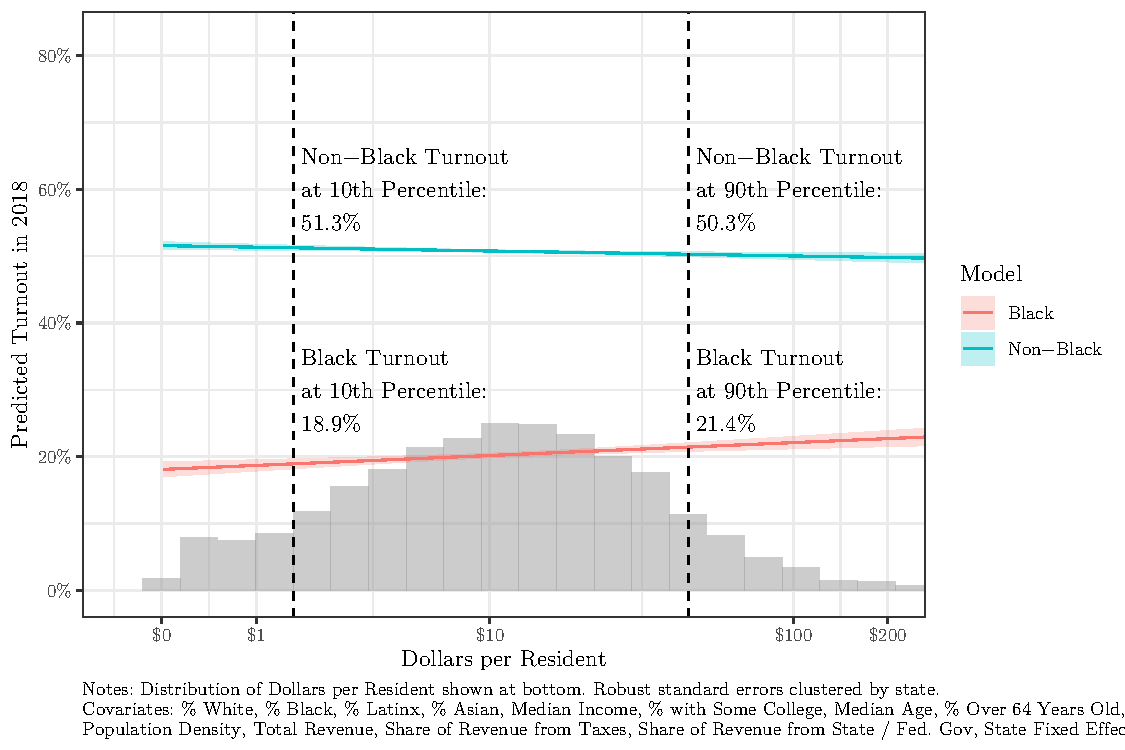
\includegraphics{draft_paper_files/figure-latex/cross-18-1} 

}

\caption{\label{fig:mef-2018}Marginal Effect of per-capita Fees and Fines on Turnout, 2018}\label{fig:cross-18}
\end{figure}

As Figure \ref{fig:mef-2018} makes clear, turnout was lower for non-Black voters in municipalities with higher fees and fines collections per resident: it dropped by roughly 1 percentage point over the interdecile range, after controlling for the other covariates. The opposite is true for Black voters: over the same range, Black turnout \emph{increases} by roughly 2.5 percentage points. Both of these relationships are statistically significant at the 95 confidence level. To be sure, this does not prove that higher fees and fines increase Black turnout; these cross-sectional regressions cannot establish causality. Nevertheless, Figure \ref{fig:mef-2018} is consistent with this story.

We turn now to our two-way fixed effects model. As discussed above, we retain each municipality that reported their fees and fines data to the COG in both 2012 and 2017 (and met the other criteria discussed in the \emph{Data and Design} section). The dependent variable in each model is calculated by dividing the number of ballots cast in 2014 and 2018 by the 5-year CVAP estimate from the same year. We run the two-way fixed effects on overall turnout, Black turnout, and non-Black turnout. The results of these models can be found in Table \ref{tab:twfe}.

\begin{singlespace}
\input{"../temp/2wfe_reg_clean.tex"}
\end{singlespace}

The results of the two-way fixed effects model are slightly different than what we saw in the 2018 cross-sectional approach; namely, while Table \ref{tab:twfe} indicates that higher fees and fines cause lower turnout among non-Black individuals, but do not impact Black turnout. The estimated coefficient, however, is small: a 10 percent increase in fees and fines is associated with a decrease in turnout of about 0.06 percentage points. Moreover, because of the relative stability in fees and fines collections at the municipal level over this time period (the mean increase in per-capita fees and fines collections was just 6 percent, and the median municipality decreased by about 1.5 percent), it is not clear how informative this approach is.

In Table \ref{tab:coarser}, we re-estimate the model from Table \ref{tab:twfe} but coarsen the data. Here, we test whether turnout changed for municipalities who increased their fees and fines collections differently than municipalities where collections stayed the same or decreased. Municipalities that increased their per-capita fees and fines are considered ``treated.''

\begin{singlespace}
\input{"../temp/coarser_reg_clean.tex"}
\end{singlespace}

The coefficient on \emph{Treated × 2018} indicates that non-Black turnout dropped by about 0.5 percentage points in municipalities where fees and fines collections increased relative to other municipalities. While this coefficient is slightly positive for Black voters, it is not statistically significantly different from 0. In other words, both Tables \ref{tab:twfe} and \ref{tab:coarser} indicate that increased fees and fines collections decrease non-Black turnout but have no impact on Black turnout.

\hypertarget{individual-level-results}{%
\subsection*{Individual-Level Results}\label{individual-level-results}}
\addcontentsline{toc}{subsection}{Individual-Level Results}

Thus far, we have shown that the turnout effects of fees and fines collection impact municipal-level turnout, and that the effects are different for Black and non-Black Americans. We argue that this relationship is causal: increased fees and fines collections means that more residents have direct interactions with the criminal legal system. Based on prior literature, we assume there are indirect effects as well, as more residents know a family or community member who has been ticketed. While the national analysis gives us great breadth and an increased understanding of how this plays out across the country, municipal-level data leaves us unable to directly observe the causal mechanisms at play.

To directly observe the effect of being ticketed on voter participation, we now turn to our individual-level analysis in Hillsborough County, Florida. As discussed above, we match (\protect\hyperlink{ref-Sekhon2011}{Sekhon 2011}) individuals who were stopped and assessed a fine between the 2012 and 2018 elections to individuals who were not stopped during this time period.\footnote{Due to computing constraints, a 5 percent random sample stratified by treatment status is used to calculate the genetic weights. The full sample is used in the actual matching process.} Matching is done with replacement and ties are not broken, meaning some treated voters may have more than 2 controls; the regression weights reflect this possibility. In Table \ref{tab:balance} we present the results of the matching algorithm. We manage to reduce between treated and control voters substantially along all observed characteristics with the exception of 2012 turnout. However, this is not likely a problem: the turnout of all potential and actual controls were both within 0.1 percentage points of the treatment group's turnout that year.

\begin{singlespace}
\begin{table}[H]

\caption{\label{tab:baltab-chunk}\label{tab:balance} Balance Table}
\centering
\resizebox{\linewidth}{!}{
\begin{tabular}[t]{lllll}
\toprule
Variable & Treated & All Untreated & Actual Controls & Mean Improvement\\
\midrule
\% White & 49.2\% & 62.3\% & 49.2\% & 99.97\%\\
\% Black & 23.1\% & 12.7\% & 23.1\% & 99.72\%\\
\% Latino & 18.8\% & 16.3\% & 18.8\% & 99.83\%\\
\% Asian & 2.2\% & 2.7\% & 2.2\% & 97.90\%\\
\% Male & 50.8\% & 43.1\% & 50.7\% & 98.29\%\\
\% Democrat & 42.0\% & 37.6\% & 42.2\% & 93.45\%\\
\% Republican & 24.6\% & 31.4\% & 24.0\% & 91.52\%\\
Age & 43.42 & 51.88 & 43.37 & 99.40\%\\
Registration Date & 2006-06-27 & 2004-08-08 & 2006-07-06 & 98.65\%\\
Stops Prior to 2012 Election & 1.31 & 0.36 & 1.31 & 99.82\%\\
Turnout in 2010 & 20.8\% & 27.2\% & 20.7\% & 97.98\%\\
Turnout in 2012 & 47.1\% & 45.5\% & 47.1\% & 99.14\%\\
Median Income & \$63,885 & \$67,952 & \$63,757 & 96.85\%\\
\% with Some College & 74.6\% & 76.6\% & 74.8\% & 90.88\%\\
Unemployment Rate & 6.5\% & 5.8\% & 6.4\% & 92.64\%\\
\bottomrule
\end{tabular}}
\end{table}
\end{singlespace}

It is worth noting that voters who were stopped between 2012 and 2018 were far more likely to be Black, males, and registered Democrats than the general electorate, and live in Census block groups with moderately lower incomes. Unsurprisingly, they were also stopped at higher rates in the pre-treatment period than those never stopped between 2012 and 2018.

While Table \ref{tab:balance} indicates that our treatment voters and their matches are substantially similar to their matches, the validity of the difference-in-differences design requires that the treatment and control voters turned out at comparable rates in the baseline period. In Figure \ref{fig:did1}, we plot the turnout of treated and control voters in the elections before and after the treated voter was stopped. The first election following a treated voter's stop is denoted as \emph{t = 0}; subsequent elections take higher positive numbers, while the years in which \emph{t} is less than zero are the periods prior to the stop. This means that for someone stopped in 2013, \emph{t} is 0 in 2014, while \emph{t} is equal to 0 in 2018 for an individual stopped between the 2016 and 2018 elections.

\begin{figure}[H]

{\centering 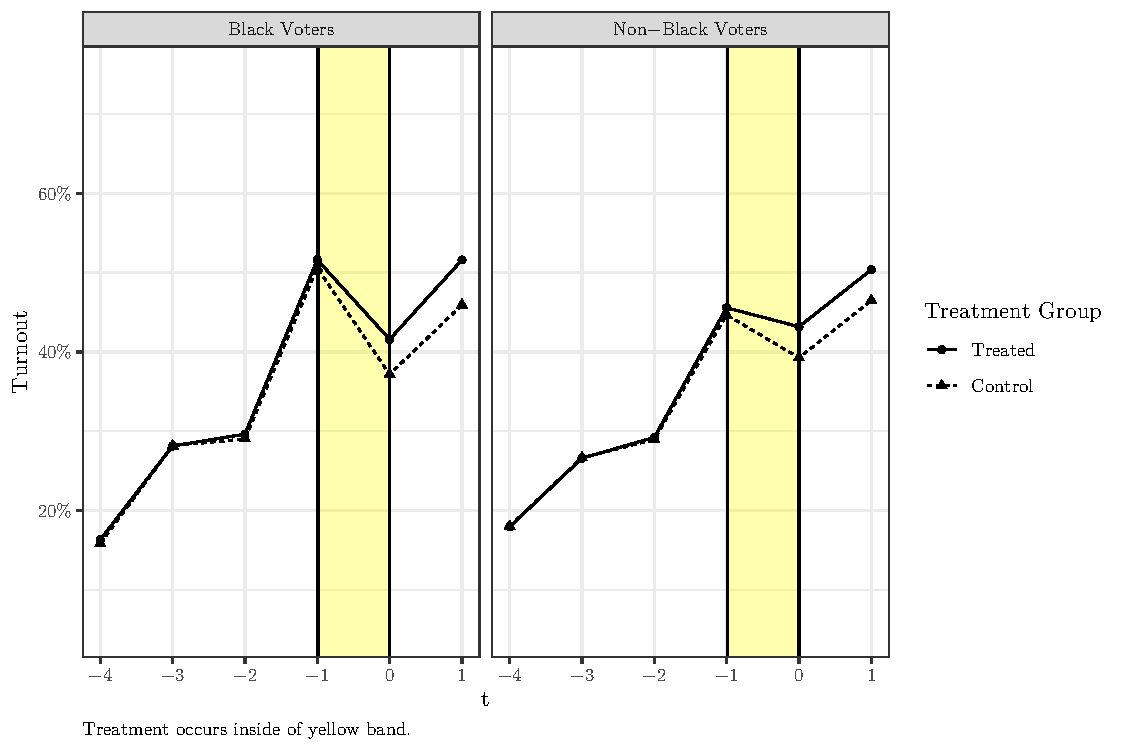
\includegraphics{draft_paper_files/figure-latex/did1-1} 

}

\caption{\label{fig:did-1}Effect of Being Ticketed on Turnout}\label{fig:did1}
\end{figure}

Figure \ref{fig:did1} makes a number of things immediately apparent. First, we can see that for both Black and non-Black voters the parallel trends assumption is satisfied. Because we matched treated and control voters based on turnout prior to the ticket, this is unsurprising. The visual results of the post-treatment trend corroborate what we found nationwide using the municipal-level data; namely, ticketing has a different effect for Black voters than for others..

Figure \ref{fig:did2} makes this effect even clearer. Here, we limit the analysis to voters who were stopped within the 90 days prior to an election (and their controls). We expected that the ticket would be more salient for individuals stopped shortly before the election. This appears to be the case --- \emph{especially for Black voters.}

\begin{figure}[H]

{\centering 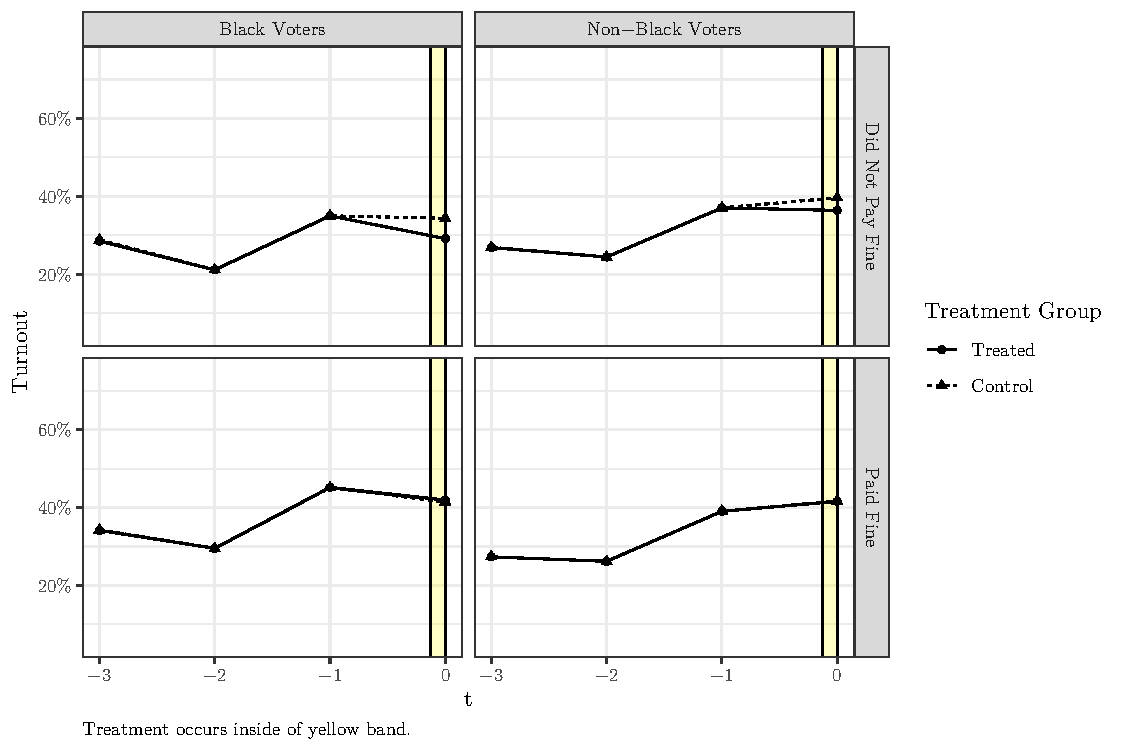
\includegraphics{draft_paper_files/figure-latex/did2-1} 

}

\caption{\label{fig:did-2}Effect of Being Ticketed Within 90 Days of Election on Turnout}\label{fig:did2}
\end{figure}

Table \ref{tab:dind-table} formalizes Figures \ref{fig:did1} and \ref{fig:did2} into an ordinary least squares regression. Models 1 and 2 present the causal estimates of being stopped at any point in the two years prior to an election; Models 3 and 4 re-estimate the effect of being stopped within 90 days of an election. Models 1 and 3 show our overall causal effect, while Models 2 and 4 allow for the possibility that a ticket differentially mobilizes Black voters. The coefficients of note are \emph{Treated × Post Treatment} and \emph{Treated × Post Treatment × Black}. In models 1 and 3, \emph{Treated × Post Treatment} measures the overall treatment effect, and in models 2 and 4 it measures the treatment effect for non-Black voters. \emph{Treated × Post Treatment × Black} measures any effect for Black voters above-and-beyond the effect measured for non-Black voters.

\begin{singlespace}
\input{"../temp/dind_reg.tex"}
\end{singlespace}

Model 3 indicates that a ticket is neither mobilizing nor demobilizing --- the coefficient is small and nonsignificant (\emph{p} = 0.34) but that tickets do mobilize Black voters. Receiving a ticket increases the average turnout for Black voters in the first two elections by about 1.1 percentage points. Model 4 shows that ticketing shortly before an election increases the turnout of non-Black voters by about 0.9 percentage points, and there is no statistically significantly different effect for Black voters. However, Figure \ref{fig:did2} visually indicates that the effect might be larger for Black voters, and the coefficient on \emph{Treated × Post Treatment × Black} is large (as is its standard error). These two facts taken together indicate that our inability to detect a differentially mobilizing effect for Black voters stopped shortly before an election may have more to do with issues of statistical power than an additional effect that is really equal to zero.

{[}Tampa - local figure/table{]}

{[}Tampa local analysis{]}

\hypertarget{discussion}{%
\subsubsection*{Discussion}\label{discussion}}
\addcontentsline{toc}{subsubsection}{Discussion}

Our results provide support for Walker's theory of criminal legal contact mobilizing nonwhite political participation. Our individual-level analysis in Hillsborough County shows that being ticketed mobilizes voters, and mobilizes Black voters to a greater degree than non-Black voters---and our city-level analysis shows that while greater fines and fees reliance reduces white voter turnout, it has no effect on Black turnout.

{[}Particularly following the rise of the Black Lives Matter movement in 2013, our findings are consistent with the theory that Black voters interpret exploitative police practices as a threat to the wellbeing of all Black Americans.{]}

We were somewhat surprised by the differences that arose between our two sets of findings---our city-level analysis did not produce statistically significant results for Black voters. We think there are a few potential explanations for this mismatch. First, compared to the individual-level analysis, our city-level analysis is much less sensitive to the temporal placement of treatment, which could explain why the city-level effect sizes are smaller or not statistically significant. Along a similar vein, it's possible that the effect size for Black voters in the city-level analysis is affected by higher-intensity forms of criminal legal contact, such as arrest and incarceration. The bulk of existing literature suggests that incarceration discourages political participation, and it's not unreasonable to assume that cities that ramp up ticketing of Black residents also ramp up arrest and incarceration of Black residents. If these phenomena coincide, that could explain why the city-level analysis produced no statistically significant effect for Black voters---the personally mobilizing effect of ticketing could be counterbalanced by the proximal chilling effect of incarceration, and because the city-level analysis is not as temporally sensitive, it's more difficult to isolate the effect of ticketing.

\textbf{Limitations}: Because our individual-level analysis is limited to Hillsborough County, we don't have a good idea of whether the city-level revenue reliance trend interacts with the individual experience of being ticketed. Is ticketing more politically mobilizing in cities that are palpably dialing up their revenue collection efforts? Future research could test this hypothesis in cities that either maintained constant fines and fees revenue reliance over time or reduced revenue reliance.

Additionally, in our analysis of Hillsborough County voters, we don't look at people who weren't registered to vote in 2018. This means that there could be some proportion of ticketed Black motorists who are now less likely to register to vote in the first place, for example. In other words the mobilization effect in our findings only applies to people who were registered to vote---we are unable to make claims about whether being ticketed makes an individual more likely to register to vote.

\textbf{Future research}: Unlike previous studies using survey data, we are unable to tell whether individuals in Tampa have non-ticketing criminal legal exposure. Future research could test whether formerly incarcerated people respond to unjust ticketing by mobilizing or withdrawing from political participation.{]}

{[}Laniyonu{]} - {[}he writes that block groups with higher Black pop and higher SQF density voted at higher rates for Thompson, the candidate who pledged not to implement SQF reform, but who was Black. The descriptive representation from Sances2017 kind of covers for this, tactically speaking - electing Black politicians should reduce fines and fees abuses. But in Tampa, the current mayor, Jane Castor, was the police chief until 2015 --- which overlaps with the treatment period in our analysis. One voter told the Tampa Bay Times that he voted against Castor as ``payback'' for the racist ticketing practices she oversaw, and the article notes that her opponent won five majority-Black precincts (\protect\hyperlink{ref-Frago2019}{Frago 2019}). In 2015, Castor even released a statement as police chief supporting the racist ticketing, insisting that ``Many individuals receiving bike citations are involved in criminal activity.''

\newpage

\hypertarget{references}{%
\section*{References}\label{references}}
\addcontentsline{toc}{section}{References}

\hypertarget{refs}{}
\begin{CSLReferences}{1}{0}
\leavevmode\hypertarget{ref-Behrens2003}{}%
Behrens, A., C. Uggen, and Jeff Manza. 2003. {``Ballot {Manipulation} and the {`{Menace} of {Negro Domination}'}: {Racial Threat} and {Felon Disenfranchisement} in the {United States}, 1850--20021.''} \emph{American Journal of Sociology}. \url{https://doi.org/10.1086/378647}.

\leavevmode\hypertarget{ref-Bell2017}{}%
Bell, Monica C. 2017. {``Police {Reform} and the {Dismantling} of {Legal Estrangement}.''} \emph{The Yale Law Journal} 126 (7): 2054--150. \url{http://www.jstor.org/stable/45222555}.

\leavevmode\hypertarget{ref-Blessett2016}{}%
Blessett, Brandi, and Richard Box. 2016. {``Sharecropper {Finance}: {Using} the {Justice System} as a {Public Revenue Source}.''} \emph{Public Integrity} 18 (January): 113--26. \url{https://doi.org/10.1080/10999922.2015.1111742}.

\leavevmode\hypertarget{ref-Brayne2014}{}%
Brayne, Sarah. 2014. {``Surveillance and {System Avoidance}: {Criminal Justice Contact} and {Institutional Attachment}.''} \emph{American Sociological Review} 79 (3): 367--91. \url{https://doi.org/10.1177/0003122414530398}.

\leavevmode\hypertarget{ref-Burch2014}{}%
Burch, Traci R. 2014. {``Effects of {Imprisonment} and {Community Supervision} on {Neighborhood Political Participation} in {North Carolina}.''} \emph{The ANNALS of the American Academy of Political and Social Science} 651 (1): 184--201. \url{https://doi.org/10.1177/0002716213503093}.

\leavevmode\hypertarget{ref-Campbell2021}{}%
Campbell, Travis. 2021. {``Black {Lives Matter}'s {Effect} on {Police Lethal Use}-of-{Force}.''} SSRN Scholarly Paper ID 3767097. {Rochester, NY}: {Social Science Research Network}. \url{https://doi.org/10.2139/ssrn.3767097}.

\leavevmode\hypertarget{ref-Carlton2018}{}%
Carlton, Sue. 2018. {``Carlton: {Jane Castor} Now Says Biking-While-Black Tickets Were Wrong.''} \emph{Tampa Bay Times}, April 12, 2018. \url{https://www.tampabay.com/news/politics/local/Carlton-Jane-Castor-now-says-biking-while-black-tickets-were-wrong_167233952/}.

\leavevmode\hypertarget{ref-CarpenterII2019}{}%
Carpenter II, Dick M, Kyle Sweetland, and Jennifer McDonald. 2019. {``The {Price} of {Taxation} by {Citation}: {Case Studies} of {Three Georgia Cities That Rely Heavily} on {Fines} and {Fees}.''} {Institute for Justice}.

\leavevmode\hypertarget{ref-Colgan2019}{}%
Colgan, Beth A. 2019. {``Wealth-{Based Penal Disenfranchisement}.''} \emph{Vanderbilt Law Review} 72 (January). \url{https://papers.ssrn.com/abstract=3312439}.

\leavevmode\hypertarget{ref-Cox2019}{}%
Cox, Kiana. 2019. {``Most {U}.{S}. Adults Feel What Happens to Their Own Racial or Ethnic Group Affects Them Personally.''} {Pew Research Center}. July 11, 2019. \url{https://www.pewresearch.org/fact-tank/2019/07/11/linked-fate-connectedness-americans/}.

\leavevmode\hypertarget{ref-Desmond2016}{}%
Desmond, Matthew, Andrew V. Papachristos, and David S. Kirk. 2016. {``Police {Violence} and {Citizen Crime Reporting} in the {Black Community}.''} \emph{American Sociological Review} 81 (5): 857--76. \url{https://doi.org/10.1177/0003122416663494}.

\leavevmode\hypertarget{ref-DuBois1935}{}%
Du Bois, W. E. B. 1935. \emph{Black {Reconstruction} in {America}}. {Harcourt, Brace, and Howe}.

\leavevmode\hypertarget{ref-Dunn2009}{}%
Dunn, Ronnie A. 2009. {``Measuring {Racial Disparities} in {Traffic Ticketing Within Large Urban Jurisdictions}.''} \emph{Public Performance \& Management Review} 32 (4): 537--61. \url{https://doi.org/10.2753/PMR1530-9576320403}.

\leavevmode\hypertarget{ref-Edwards2020}{}%
Edwards, Frank, and Alexes Harris. 2020. {``An {Analysis} of {Court Imposed Monetary Sanctions} in {Seattle Municipal Courts}, 2000-2017.''} August. \url{https://doi.org/10.31235/osf.io/ajpqc}.

\leavevmode\hypertarget{ref-Frago2019}{}%
Frago, Charlie. 2019. {``Tampa Police Have {`Evolved'} on Biking While Black, Chief Says.''} \emph{Tampa Bay Times}, October 24, 2019. \url{https://www.tampabay.com/news/tampa/2019/10/24/tampa-police-have-evolved-on-biking-while-black-chief-says/}.

\leavevmode\hypertarget{ref-Friedman2020}{}%
Friedman, Brittany. 2020. {``Carceral {Immobility} and {Financial Capture}: {A Framework} for the {Consequences} of {Racial Capitalism Penology} and {Monetary Sanctions}.''} \emph{UCLA Criminal Justice Law Review} 4 (1). \url{https://escholarship.org/uc/item/31r669wf}.

\leavevmode\hypertarget{ref-Gilmore2007}{}%
Gilmore, Ruth Wilson. 2007. \emph{Golden {Gulag}: {Prisons}, {Surplus}, {Crisis}, and {Opposition} in {Globalizing California}}. {University of California Press}.

\leavevmode\hypertarget{ref-Goldstein2020}{}%
Goldstein, Rebecca, Michael W. Sances, and Hye Young You. 2020. {``Exploitative {Revenues}, {Law Enforcement}, and the {Quality} of {Government Service}.''} \emph{Urban Affairs Review} 56 (1): 5--31. \url{https://doi.org/10.1177/1078087418791775}.

\leavevmode\hypertarget{ref-Goncalves2020}{}%
Goncalves, Felipe, and Steven Mello. 2020. {``A {Few Bad Apples}? {Racial Bias} in {Policing}.''} SSRN Scholarly Paper ID 3627809. {Rochester, NY}: {Social Science Research Network}. \url{https://doi.org/10.2139/ssrn.3627809}.

\leavevmode\hypertarget{ref-BoardofGovernorsoftheFederalReserveSystem2020}{}%
Governors of the Federal Reserve System, Board of. 2020. {``Report on the {Economic Well}-{Being} of {U}.{S}. {Households} in 2019, {Featuring Supplemental Data} from {April} 2020.''} {Federal Reserve System}. \url{https://www.federalreserve.gov/publications/report-economic-well-being-us-households.htm}.

\leavevmode\hypertarget{ref-Hadden2003}{}%
Hadden, Sally. 2003. \emph{Slave {Patrols}}. \url{https://www.hup.harvard.edu/catalog.php?isbn=9780674012349}.

\leavevmode\hypertarget{ref-Harris2010}{}%
Harris, Alexes, Heather Evans, and Katherine Beckett. 2010. {``Drawing {Blood} from {Stones}: {Legal Debt} and {Social Inequality} in the {Contemporary United States}.''} \emph{American Journal of Sociology} 115 (6): 1753--99. \url{https://doi.org/10.1086/651940}.

\leavevmode\hypertarget{ref-Harris2011}{}%
---------. 2011. {``Courtesy {Stigma} and {Monetary Sanctions}: {Toward} a {Socio}-{Cultural Theory} of {Punishment}.''} \emph{American Sociological Review} 76 (2): 234--64. \url{https://doi.org/10.1177/0003122411400054}.

\leavevmode\hypertarget{ref-Harris2017}{}%
Harris, Alexes, Beth Huebner, Karin Martin, Mary Pattillo, Becky Pettit, Sarah Shannon, Bryan Sykes, Chris Uggen, and April Fernandes. 2017. {``Monetary {Sanctions} in the {Criminal Justice System}.''}

\leavevmode\hypertarget{ref-Hinton2017}{}%
Hinton, Elizabeth. 2017. \emph{From the {War} on {Poverty} to the {War} on {Crime}: {The Making} of {Mass Incarceration} in {America}}. {Harvard University Press}.

\leavevmode\hypertarget{ref-Hinton2021}{}%
Hinton, Elizabeth, and DeAnza Cook. 2021. {``The {Mass Criminalization} of {Black Americans}: {A Historical Overview}.''} \emph{Annual Review of Criminology} 4 (1): 261--86. \url{https://doi.org/10.1146/annurev-criminol-060520-033306}.

\leavevmode\hypertarget{ref-EqualJusticeInitiative2017}{}%
Initiative, Equal Justice. 2017. {``Lynching in {America}: {Confronting} the {Legacy} of {Racial Terror}.''} \url{https://lynchinginamerica.eji.org/report/}.

\leavevmode\hypertarget{ref-Justice2014}{}%
Justice, Benjamin, and Tracey L. Meares. 2014. {``How the {Criminal Justice System Educates Citizens}.''} \emph{The ANNALS of the American Academy of Political and Social Science} 651 (1): 159--77. \url{https://doi.org/10.1177/0002716213502929}.

\leavevmode\hypertarget{ref-Kirk2020}{}%
Kirk, Gabriela, April Fernandes, and Brittany Friedman. 2020. {``Who {Pays} for the {Welfare State}? {Austerity Politics} and the {Origin} of {Pay}-to-{Stay Fees} as {Revenue Generation}.''} \emph{Sociological Perspectives} 63 (6): 921--38. \url{https://doi.org/10.1177/0731121420967037}.

\leavevmode\hypertarget{ref-Laniyonu2019}{}%
Laniyonu, Ayobami. 2019. {``The {Political Consequences} of {Policing}: {Evidence} from {New York City}.''} \emph{Political Behavior} 41 (2): 527--58. \url{https://doi.org/10.1007/s11109-018-9461-9}.

\leavevmode\hypertarget{ref-Lee2014}{}%
Lee, Hedwig, Lauren C. Porter, and Megan Comfort. 2014. {``Consequences of {Family Member Incarceration}: {Impacts} on {Civic Participation} and {Perceptions} of the {Legitimacy} and {Fairness} of {Government}.''} \emph{The ANNALS of the American Academy of Political and Social Science} 651 (1): 44--73. \url{https://doi.org/10.1177/0002716213502920}.

\leavevmode\hypertarget{ref-Lerman2014}{}%
Lerman, Amy E., and Vesla M. Weaver. 2014. \emph{Arresting Citizenship: The Democratic Consequences of {American} Crime Control}. Chicago Studies in {American} Politics. {Chicago ; London}: {The University of Chicago Press}.

\leavevmode\hypertarget{ref-Lichtenstein1996}{}%
Lichtenstein, Alexander C. 1996. \emph{Twice the {Work} of {Free Labor}}. {Verso}. \url{https://www.versobooks.com/books/738-twice-the-work-of-free-labor}.

\leavevmode\hypertarget{ref-Makowsky2009}{}%
Makowsky, Michael D., and Thomas Stratmann. 2009. {``Political {Economy} at {Any Speed}: {What Determines Traffic Citations}?''} \emph{The American Economic Review} 99 (1): 509--27. \url{http://www.jstor.org/stable/29730194}.

\leavevmode\hypertarget{ref-Mancini1978}{}%
Mancini, Matthew J. 1978. {``Race, {Economics}, and {The Abandonment} of {Convict Leasing}.''} \emph{The Journal of Negro History} 63 (4): 339--52. \url{https://doi.org/10.2307/2716851}.

\leavevmode\hypertarget{ref-Martin2017}{}%
Martin, Isaac William, and Kevin Beck. 2017. {``Property {Tax Limitation} and {Racial Inequality} in {Effective Tax Rates}.''} \emph{Critical Sociology} 43 (2): 221--36. \url{https://doi.org/10.1177/0896920515607073}.

\leavevmode\hypertarget{ref-Meares2017}{}%
Meares, Tracey. 2017. {``Policing and {Procedural Justice}: {Shaping Citizens}' {Identities} to {Increase Democratic Participation}.''} \emph{Northwestern University Law Review} 111 (6): 1525--36.

\leavevmode\hypertarget{ref-Meredith2014}{}%
Meredith, Marc, and Michael Morse. 2014. {``Do {Voting Rights Notification Laws Increase Ex}-{Felon Turnout}?''} \emph{The ANNALS of the American Academy of Political and Social Science} 651 (1): 220--49. \url{https://doi.org/10.1177/0002716213502931}.

\leavevmode\hypertarget{ref-Meredith2017}{}%
---------. 2017. {``Discretionary {Disenfranchisement}: {The Case} of {Legal Financial Obligations}.''} \emph{The Journal of Legal Studies} 46 (2): 309--38. \url{https://doi.org/10.1086/694323}.

\leavevmode\hypertarget{ref-Morris2020}{}%
Morris, Kevin. 2020. {``Neighborhoods and {Felony Disenfranchisement}: {The Case} of {New York City}.''} \emph{Urban Affairs Review}, May, 1078087420921522. \url{https://doi.org/10.1177/1078087420921522}.

\leavevmode\hypertarget{ref-Mughan2020}{}%
Mughan, Siân. 2020. {``Municipal {Reliance} on {Fine} and {Fee Revenues}: {How Local Courts Contribute} to {Extractive Revenue Practices} in {U}.{S}. {Cities}.''} \emph{Public Budgeting \& Finance}, December. \url{https://doi.org/10.1111/pbaf.12277}.

\leavevmode\hypertarget{ref-Muhammad2010}{}%
Muhammad, Khalil Gibran. 2010. \emph{The {Condemnation} of {Blackness} --- {Khalil Gibran Muhammad} \textbar{} {Harvard University Press}}. {Harvard University Press}. \url{https://www.hup.harvard.edu/catalog.php?isbn=9780674238145}.

\leavevmode\hypertarget{ref-Nyhan2017}{}%
Nyhan, Brendan, Christopher Skovron, and Rocío Titiunik. 2017. {``Differential {Registration Bias} in {Voter File Data}: {A Sensitivity Analysis Approach}.''} \emph{American Journal of Political Science} 61 (3): 744--60. \url{https://doi.org/10.1111/ajps.12288}.

\leavevmode\hypertarget{ref-Pacewicz2020}{}%
Pacewicz, Josh, and John N.Robinson III. 2020. {``Pocketbook Policing: {How} Race Shapes Municipal Reliance on Punitive Fines and Fees in the {Chicago} Suburbs.''} \emph{Socio-Economic Review}, October. \url{https://doi.org/10.1093/ser/mwaa029}.

\leavevmode\hypertarget{ref-Pierson2020}{}%
Pierson, Emma, Camelia Simoiu, Jan Overgoor, Sam Corbett-Davies, Daniel Jenson, Amy Shoemaker, Vignesh Ramachandran, et al. 2020. {``A Large-Scale Analysis of Racial Disparities in Police Stops Across the {United States}.''} \emph{Nature Human Behaviour} 4 (7, 7): 736--45. \url{https://doi.org/10.1038/s41562-020-0858-1}.

\leavevmode\hypertarget{ref-Remster2018}{}%
Remster, Brianna, and Rory Kramer. 2018/ed. {``{SHIFTING POWER}: {The Impact} of {Incarceration} on {Political Representation}.''} \emph{Du Bois Review: Social Science Research on Race} 15 (2): 417--39. \url{https://doi.org/10.1017/S1742058X18000206}.

\leavevmode\hypertarget{ref-Remster2018a}{}%
---------. 2018. {``Race, {Space}, and {Surveillance}: {Understanding} the {Relationship} Between {Criminal Justice Contact} and {Institutional Involvement}.''} \emph{Socius} 4 (January). \url{https://doi.org/10.1177/2378023118761434}.

\leavevmode\hypertarget{ref-Robinson2000}{}%
Robinson, Cedric J. 2000. \emph{Black {Marxism}: The {Making} of the {Black Radical Tradition}}. {University of North Carolina Press}. \url{https://uncpress.org/book/9780807848296/black-marxism/}.

\leavevmode\hypertarget{ref-Rothstein2017}{}%
Rothstein, Richard. 2017. \emph{The Color of Law: A Forgotten History of How Our Government Segregated {America}}. First edition. {New York ; London}: {Liveright Publishing Corporation, a division of W. W. Norton \& Company}.

\leavevmode\hypertarget{ref-Sances2017}{}%
Sances, Michael W., and Hye Young You. 2017. {``Who {Pays} for {Government}? {Descriptive Representation} and {Exploitative Revenue Sources}.''} \emph{The Journal of Politics} 79 (3): 1090--94. \url{https://doi.org/10.1086/691354}.

\leavevmode\hypertarget{ref-Sekhon2011}{}%
Sekhon, Jasjeet S. 2011. {``Multivariate and {Propensity Score Matching Software} with {Automated Balance Optimization}: {The Matching} Package for {R}.''} \emph{Journal of Statistical Software} 42 (7): 1--52. \url{https://doi.org/10.18637/jss.v042.i07}.

\leavevmode\hypertarget{ref-Shofner1963}{}%
Shofner, Jerrell H. 1963. {``The {Constitution} of 1868.''} \emph{The Florida Historical Quarterly} 41 (4): 356--74. \url{http://www.jstor.org/stable/30139965}.

\leavevmode\hypertarget{ref-Singla2020}{}%
Singla, Akheil, Charlotte Kirschner, and Samuel B. Stone. 2020. {``Race, {Representation}, and {Revenue}: {Reliance} on {Fines} and {Forfeitures} in {City Governments}.''} \emph{Urban Affairs Review} 56 (4): 1132--67. \url{https://doi.org/10.1177/1078087419834632}.

\leavevmode\hypertarget{ref-Sugie2015}{}%
Sugie, Naomi F. 2015. {``Chilling {Effects}: {Diminished Political Participation} Among {Partners} of {Formerly Incarcerated Men}.''} \emph{Social Problems} 62 (4): 550--71. \url{http://www.jstor.org/stable/44014875}.

\leavevmode\hypertarget{ref-Tyler2014}{}%
Tyler, Tom R., Jeffrey Fagan, and Amanda Geller. 2014. {``Street {Stops} and {Police Legitimacy}: {Teachable Moments} in {Young Urban Men}'s {Legal Socialization}.''} \emph{Journal of Empirical Legal Studies} 11 (4): 751--85. \url{https://doi.org/10.1111/jels.12055}.

\leavevmode\hypertarget{ref-Uggen2020}{}%
Uggen, Christopher, Ryan Larson, Sarah Shannon, and Arleth Pulido-Nava. 2020. {``Locked {Out} 2020: {Estimates} of {People Denied Voting Rights Due} to a {Felony Conviction}.''} Research report. {The Sentencing Project}. \url{https://www.sentencingproject.org/wp-content/uploads/2020/10/Locked-Out-2020.pdf}.

\leavevmode\hypertarget{ref-UnitedStatesCommissiononCivilRights2017}{}%
United States Commission on Civil Rights. 2017. {``Targeted {Fines} and {Fees Against Communities} of {Color}.''} \url{https://www.usccr.gov/pubs/2017/Statutory_Enforcement_Report2017.pdf}.

\leavevmode\hypertarget{ref-UnitedStatesDepartmentofJusticeCivilRightsDivision2015}{}%
United States Department of Justice Civil Rights Division. 2015. {``Investigation of the {Ferguson Police Department}.''} \url{https://www.justice.gov/sites/default/files/opa/press-releases/attachments/2015/03/04/ferguson_police_department_report.pdf}.

\leavevmode\hypertarget{ref-Vargas2017a}{}%
Vargas, Robert, and Philip McHarris. 2017. {``Race and {State} in {City Police Spending Growth}: 1980 to 2010.''} \emph{Sociology of Race and Ethnicity} 3 (1): 96--112. \url{https://doi.org/10.1177/2332649216650692}.

\leavevmode\hypertarget{ref-Walker2014}{}%
Walker, Hannah L. 2014. {``Extending the {Effects} of the {Carceral State}: {Proximal Contact}, {Political Participation}, and {Race}.''} \emph{Political Research Quarterly}, July. \url{https://doi.org/10.1177/1065912914542522}.

\leavevmode\hypertarget{ref-Walker2020}{}%
---------. 2020. {``Targeted: {The Mobilizing Effect} of {Perceptions} of {Unfair Policing Practices}.''} \emph{The Journal of Politics} 82 (1): 119--34. \url{https://doi.org/10.1086/705684}.

\leavevmode\hypertarget{ref-Walker2017}{}%
Walker, Hannah L., and Marcela García-Castañon. 2017. {``For {Love} and {Justice}: {The Mobilizing} of {Race}, {Gender}, and {Criminal Justice Contact}.''} \emph{Politics \& Gender} 13 (4): 541--68. \url{https://doi.org/10.1017/S1743923X17000198}.

\leavevmode\hypertarget{ref-Weaver2010}{}%
Weaver, Vesla M., and Amy E. Lerman. 2010. {``Political {Consequences} of the {Carceral State}.''} \emph{American Political Science Review} 104 (4): 817--33. \url{https://doi.org/10.1017/S0003055410000456}.

\leavevmode\hypertarget{ref-White2019}{}%
White, Ariel. 2019. {``Family {Matters}? {Voting Behavior} in {Households} with {Criminal Justice Contact}.''} \emph{American Political Science Review} 113 (2): 607--13. \url{https://doi.org/10.1017/S0003055418000862}.

\leavevmode\hypertarget{ref-Zayas2015}{}%
Zayas, Alexandra. 2015. {``How Riding Your Bike Can Land You in Trouble with the Cops --- If You're Black.''} \emph{Tampa Bay Times}, April 15, 2015. \url{https://www.tampabay.com/news/publicsafety/how-riding-your-bike-can-land-you-in-trouble-with-the-cops—if-youre-black/2225966/}.

\end{CSLReferences}

\end{document}
